\section{Transport Layer}

\begin{description}
	\item schliesst Lücke zwischen IP \& Applikation
	\item[UDP] effiziente, schlanke Übertragung (verbindungslos)
	\item[TCP] zuverlässige Übertragung (verbindungsorientiert)
\end{description}

\subsubsection{Kapselung}

Applikationdaten werden mittels Transport Layer in ein IP-Paket gekapselt.

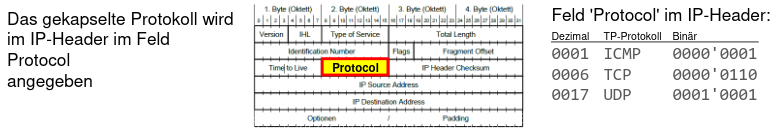
\includegraphics[width=0.9\linewidth]{tcp-ip-encap}



\subsection{Port Nummern}

\begin{itemize}
	\item einzelne Applikationen auf den Hosts werden durch Ports identifiziert
	      (de-/multiplexen)
	\item jedes TCP/UDP Paket enthält source \& destination port
\end{itemize}

\begin{center}
	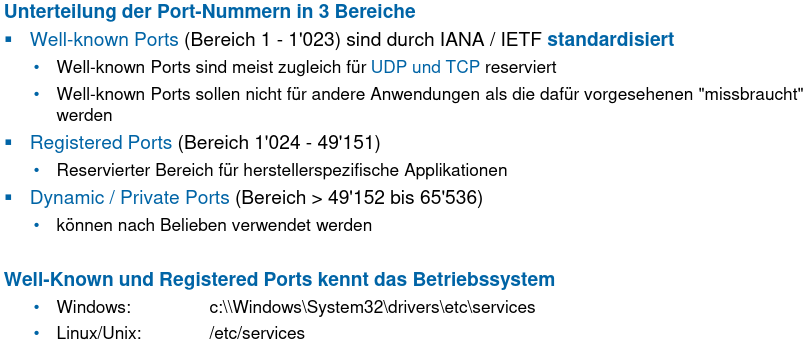
\includegraphics[width=0.9\linewidth]{tl-port-ranges}
\end{center}

\subsubsection{geläufige Well-known Ports}

\begin{center}
	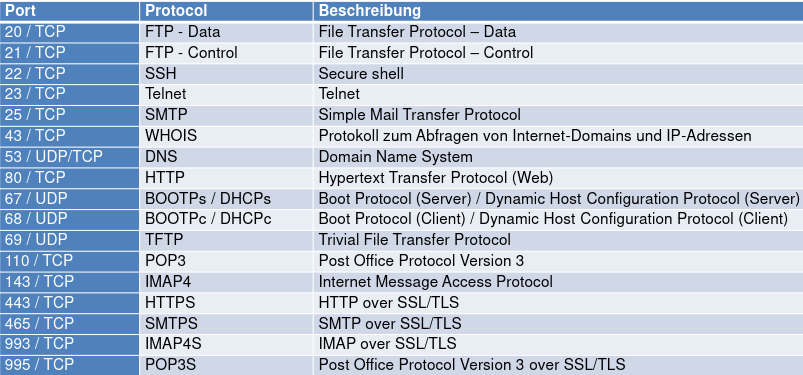
\includegraphics[width=0.9\linewidth]{tl-well-known-ports}
\end{center}



\subsection{UDP - User Datagram Protocol}

\begin{description}
	\item[Verbindungslos] Daten werden in UDP Datagramme eingefügt und direkt gesendet
	\item[Unzuverlässig] keine Massnahmen gegen Verlust oder Vertauschen
		(gleich wie IP Pakete)
\end{description}

\subsubsection{UDP Header}
\begin{center}
	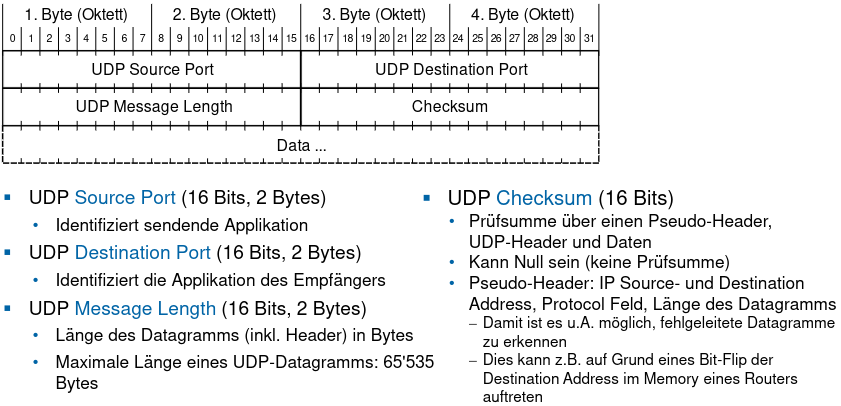
\includegraphics[width=0.9\linewidth]{tl-udp-header}
\end{center}



\subsection{TCP - Transmission Control Protocol}

\begin{description}
	\item[Verbindungsorientiert] vor Datenaustausch ist Verbindungsaufbau nötig
	\item[Zuverlässiger Verbindungsaufbau] beide Endpunkte müssen den Verbindungsaufbau
		aktiv bestätigen
	\item[Hohe Zuverlässigkeit] kein Datenverlust \& richtige Reihenfolge
	\item[Vollduplex] gleichzeitige, unabhängige Übertragung in beide Richtungen
	\item[Punkt zu Punkt] immer direkt zwei Applikationen / kein Broad-/Multicast
\end{description}

\subsubsection{TCP Nachrichtenaustausch}
In beide Richtungen:
\begin{description}
	\item[Sequence Numbers] für \textcolor{blue}{gesendete} Bytes,
		Position der Datenbytes im Gesamtstrom
		\begin{itemize}
			\item richtige Reihenfolge der Daten
			\item verlorene Daten erkennen
		\end{itemize}
	\item[Acknowledge Numbers] für \textcolor{blue}{empfangene} Bytes
		(von der anderen Seite), Sequence Number der nächsten erwarten Bytes
		\begin{itemize}
			\item Bestätigung korrekt empfangener Daten
			\item verlorene Daten erkennen
		\end{itemize}
	\item[Flags] steuern Verbindugsauf-/abbau, signalisieren Gültigkeit von Infos
		im Header und besondere Situationen
		\begin{description}
			\item[SYN/FIN] Verbindungsauf-/abbau
			\item[ACK] Acknowledge Number im emfpangen Segment ist gültig
			\item[PSH] Daten sollen schnellstmöglich an Applikation weitergeben werden
		\end{description}
\end{description}

\begin{center}
	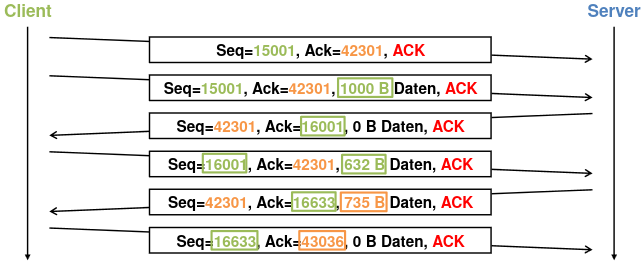
\includegraphics[width=0.9\linewidth,height=27mm]{tl-tcp-data-exchange}
\end{center}

\subsubsection{TCP Verbindungsaufbau}

\begin{center}
	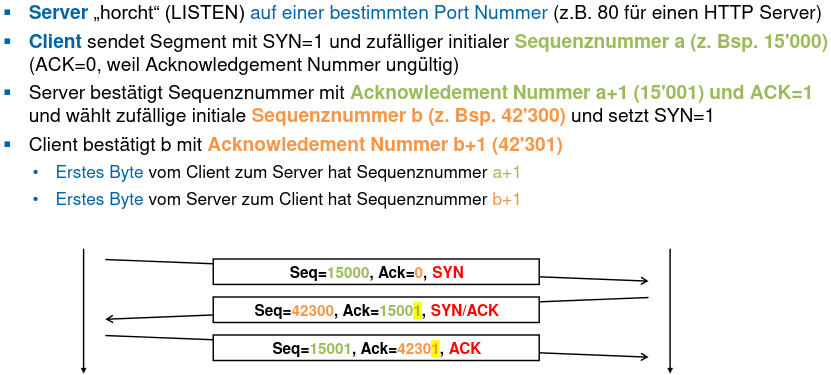
\includegraphics[width=0.95\linewidth]{tl-tcp-conn-establ}
\end{center}


\subsubsection{TCP Zustandsdiagramm}

\begin{itemize}
	\item TCP State machine existiert auf Client \& Server
	\item Applikationen ändern state via
	      \lstinline[language=C]{listen(); connect(); close()}
	\item die State Machines signalisieren sich Events mit den SYN, ACK, FIN flags
\end{itemize}


Verbindungsaufbau:
\begin{center}
	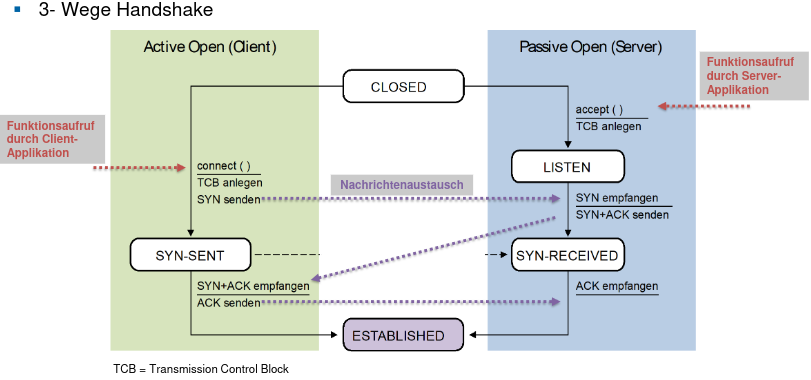
\includegraphics[width=\linewidth]{tl-tcp-state-establ}
\end{center}

Verbindungsabbau:
% TODO wieso time-wait?
\begin{center}
	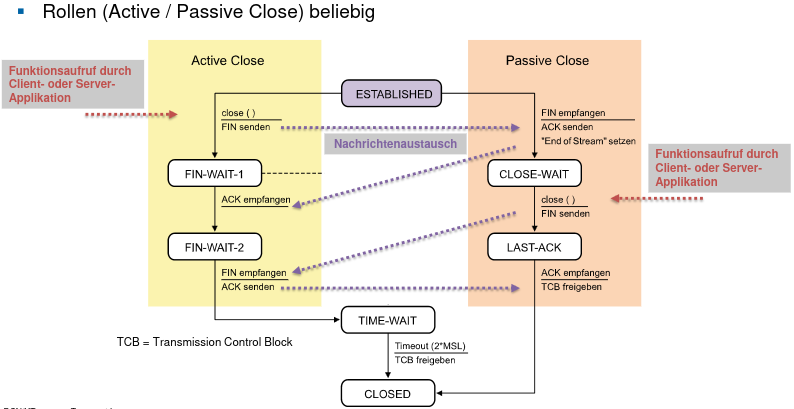
\includegraphics[width=\linewidth]{tl-tcp-state-close}
\end{center}

\subsubsection{Verlorene Nachrichten Erkennen / Retransmission-Timeout (RTO)}

Stop \& Wait:
\begin{center}
	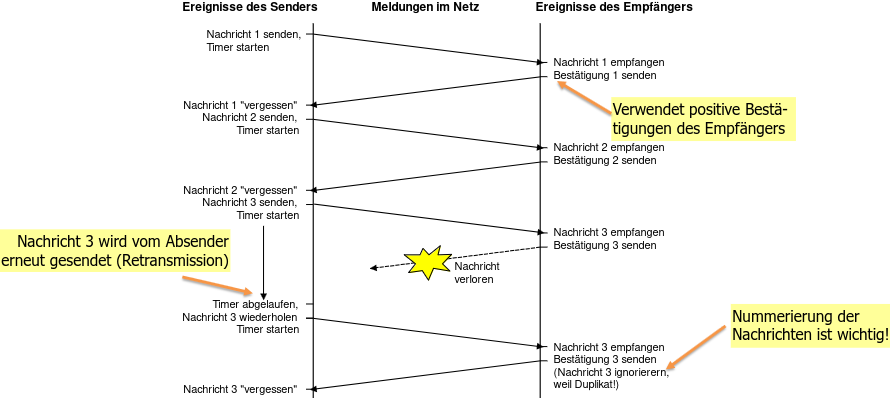
\includegraphics[width=\linewidth]{tl-tcp-stop-n-wait}
\end{center}

Vor/Nachteile:
\begin{itemize}
	\item[+] keine Überlast beim Empfänger weil Sender zuerst warten muss
	\item[-] Retransmission-Timeout(RTO) ist hoch variabel anhand von Netzwerkbedingungen.
		Zur Linderung misst TCP Round-Trip-Time (RTT) und berechnet gewichteten Mittelwert
		mit Streuung für idealen RTO
	\item[-] viel Zeit mit warten verbracht
\end{itemize}

Berechnug des RTO anhand gemessener Round-Trip-Time:
\begin{itemize}
	\item gewichteter Mittelwert SRTT (Smoothed Round-Trip-Time)\\
	      $\mathit{SRTT} = (1 - \alpha) * \mathit{SRTT} + \alpha * \mathit{RTT}
		      \quad | \quad \alpha = 0.125$
	\item Streuung RTTVAR, gewichteter Mittelwert der Abweichungen\\
	      $\mathit{RTTVAR} = (1 - \beta) * RTTVAR + \beta * |\mathit{SRTT} - \mathit{RTT}|
		      \quad | \quad \beta = 0.25$
	\item Retransmission-Timeout RTO\\
	      $\mathit{RTO} = \mathit{SRTT} + 4 * \mathit{RTTVAR}$
\end{itemize}



\subsubsection{TCP Flow-Control / Sliding Window}

Weil bei Stop \& Wait zuviel Zeit mit Warten/Netzwerklatenz verschwendet wird
$\rightarrow$ mehrere Pakete direkt nacheinander schicken solange diese ins
Fenster passen (\& nicht durch Congestion Window limitiert).

\begin{itemize}
	\item beide Seiten haben eigenes Fenster
	\item Fenstergrösse wird in Anzahl Bytes kommuniziert
	\item initiale Fenstergrösse wird bei Verbindungsaufbau mittgeteilt
	\item bei jedem ACK wird der verfügbare Fensterplatz (Bytes) mittgeteilt
	      $\rightarrow$ Fenstergrösse = 0 heisst keine Daten mehr senden
\end{itemize}

\begin{center}
	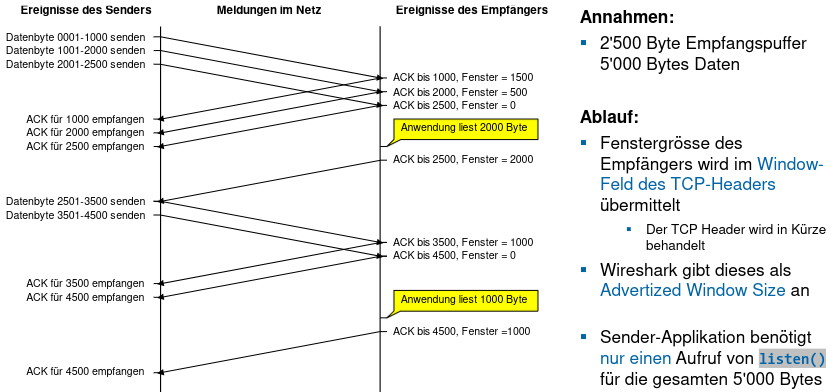
\includegraphics[width=\linewidth]{tl-tcp-sliding-window-ex}
\end{center}


\subsubsection{TCP Congestion Control}

Flow-Control schützt nur jeweils einen Empfänger, Congestion Control soll das Netz
an sich vor Überlast schützen.

Mögliche Lösung: Slow Start (unter der Annahme, dass Überlast die meisten Fehler
verursacht)

\begin{center}
	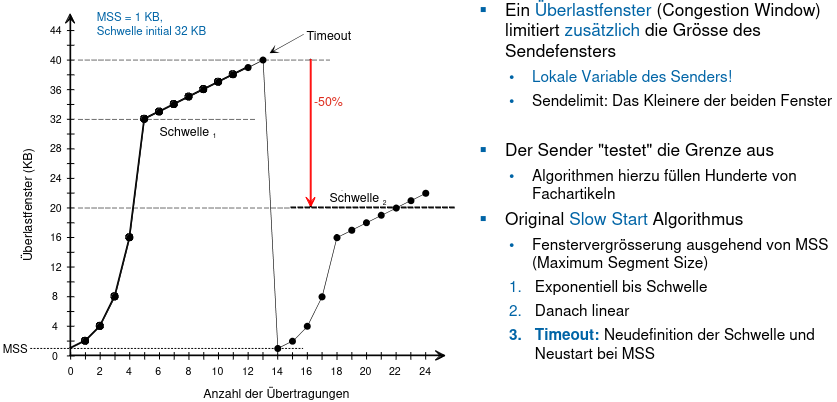
\includegraphics[width=\linewidth]{tl-tcp-cong-control-slow-start}
\end{center}


Kritikpunkte von Slow Start:
\begin{itemize}
    \item ''Sägezahnkurven'' verschiedener Session neigen sich zu synchronisieren
    \item Bei Wi-Fi sind bitfehler das grösste Problem, nicht Überlast
    \item effektiv Stop \& Wait bei kleinem Congestion Window
    \item für kurze Sessions immer langsam
    \item abhängig von Round-Trip-Time
\end{itemize}


\subsubsection{TCP Header}

\begin{center}
	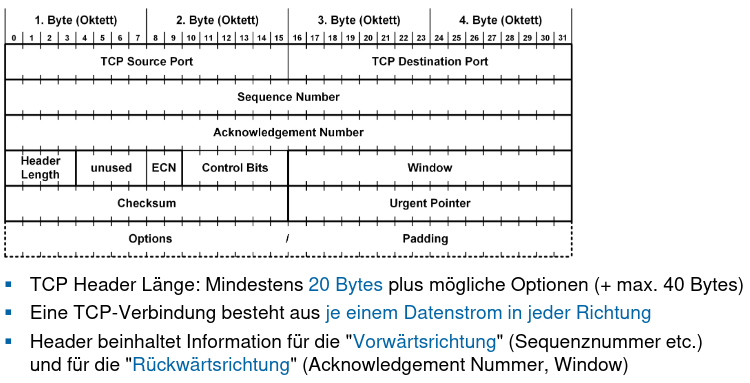
\includegraphics[width=\linewidth]{tl-tcp-header}
\end{center}

